\documentclass[tikz,border=6pt]{standalone}
\usepackage{lmodern}
\usepackage[T1]{fontenc}
\usepackage{amssymb}
\usepackage{amsmath}
\usetikzlibrary{arrows.meta,shapes.geometric,fit,backgrounds,calc,positioning,decorations.pathreplacing,patterns,matrix}
\definecolor{letterA}{HTML}{1F5FA9}
\definecolor{letterB}{HTML}{B5651D}
\definecolor{boxline}{HTML}{B9BEC4}
\definecolor{boxfill}{HTML}{F4F5F7}
\definecolor{fiberF}{HTML}{DCE6F4}
\definecolor{fiberN}{HTML}{F4E7D6}
\definecolor{perm}{HTML}{2E7D46}
\definecolor{xfail}{HTML}{C1443C}
\definecolor{hatch}{HTML}{8A9099}
\definecolor{accept}{HTML}{3A3F45}
\definecolor{ref}{HTML}{8A9099}
\definecolor{ink}{HTML}{222629}
\tikzset{
  % ---- classes ---------------------------------------------------
  cls/.style        = {circle, draw=ink, line width=.5pt, fill=white,
                       inner sep=0pt, minimum size=12mm, align=center,
                       font=\small},
  accpt/.style      = {cls, double, double distance=1pt, draw=accept},
  unit/.style       = {cls, fill=boxfill},
  % ---- λ-fibers (FIG-1 left) -------------------------------------
  fibF/.style       = {rounded corners=4pt, draw=letterA, fill=fiberF,
                       line width=.7pt},
  fibN/.style       = {rounded corners=4pt, draw=letterB, fill=fiberN,
                       line width=.7pt},
  mint/.style       = {rounded corners=2pt, draw=ink, fill=white,
                       line width=.5pt, inner sep=2pt, font=\small\ttfamily,
                       minimum width=10mm, minimum height=6mm},
  % ---- alphabet / Cayley edges -----------------------------------
  ea/.style         = {draw=letterA, text=letterA, line width=.9pt,
                       -{Stealth[length=2mm]}},
  eb/.style         = {draw=letterB, text=letterB, line width=.9pt,
                       dashed, dash pattern=on 2.4pt off 1.6pt,
                       -{Stealth[length=2mm]}},
  eall/.style       = {draw=ink, text=ink, line width=.9pt,
                       -{Stealth[length=2mm]}},
  elab/.style       = {font=\scriptsize, inner sep=1.5pt,
                       fill=white, fill opacity=.85, text opacity=1},
  % ---- the signed-permutation action -----------------------------
  perm/.style       = {draw=perm, text=perm, line width=1.1pt,
                       {Stealth[length=2mm]}-{Stealth[length=2mm]}},
  permd/.style      = {perm, dash pattern=on 3pt off 2pt},
  permlab/.style    = {font=\scriptsize, text=perm, inner sep=1.5pt,
                       fill=white, fill opacity=.85, text opacity=1},
  % ---- read-off decorations --------------------------------------
  grpbox/.style     = {rounded corners=3pt, draw=accept, line width=1.1pt},
  grptag/.style     = {font=\scriptsize\bfseries, text=accept},
  tag/.style        = {font=\scriptsize\itshape, text=ref, align=center},
  ktag/.style       = {font=\scriptsize, text=perm, align=center},
  fail/.style       = {font=\scriptsize\itshape, text=xfail, align=center},
  celltab/.style    = {font=\small\ttfamily, text=ink, inner sep=2pt},
  hdr/.style        = {font=\small\bfseries, text=ink},
}

\begin{document}
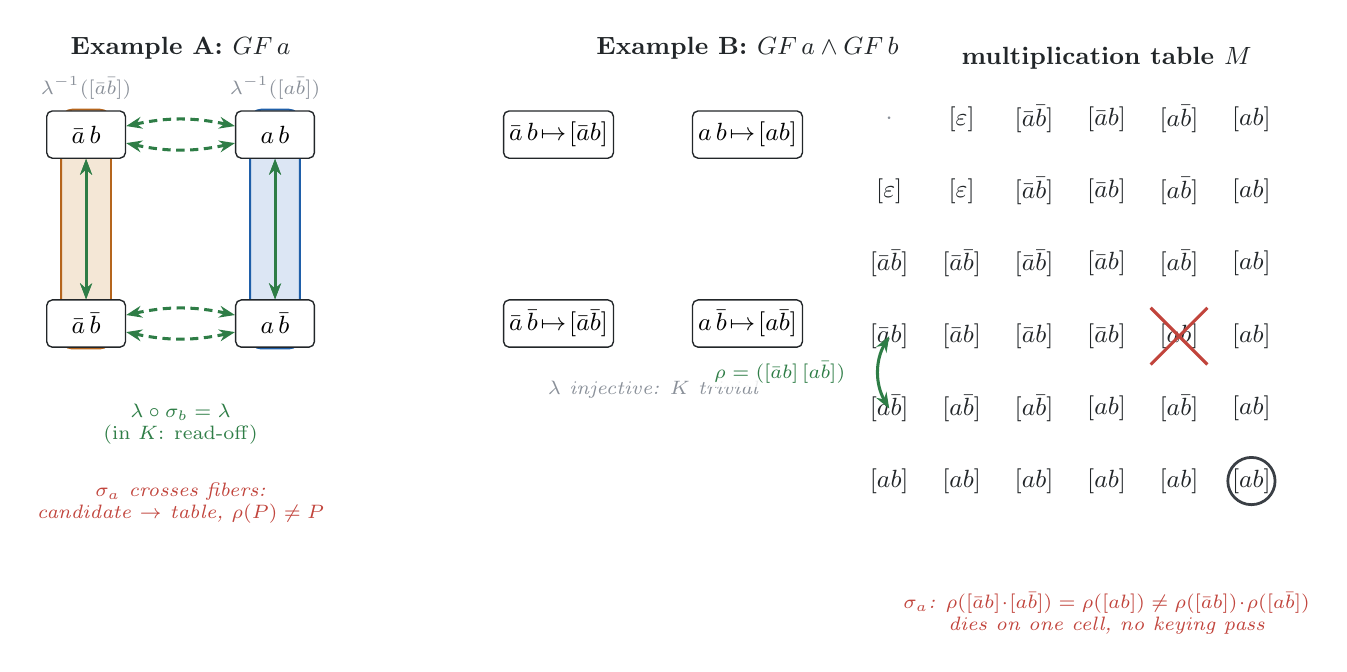
\begin{tikzpicture}
\node[hdr] at (1.20, 3.5) {Example A: $GF\,a$};
\begin{scope}[on background layer]
\coordinate (mA0) at (0.00, 0.00);
\coordinate (mA1) at (0.00, 2.40);
\node[fibN, fit=(mA0) (mA1), inner sep=9pt] (fibbox1) {};
\coordinate (mA2) at (2.40, 0.00);
\coordinate (mA3) at (2.40, 2.40);
\node[fibF, fit=(mA2) (mA3), inner sep=9pt] (fibbox2) {};
\end{scope}
\node[tag, anchor=south] at (fibbox1.north) {$\lambda^{-1}([\bar a\bar b])$};
\node[tag, anchor=south] at (fibbox2.north) {$\lambda^{-1}([a\bar b])$};
\node[mint] (mv0) at (0.00, 0.00) {$\bar a\,\bar b$};
\node[mint] (mv1) at (0.00, 2.40) {$\bar a\,b$};
\node[mint] (mv2) at (2.40, 0.00) {$a\,\bar b$};
\node[mint] (mv3) at (2.40, 2.40) {$a\,b$};
\draw[perm] (mv0) -- (mv1);
\draw[perm] (mv1) -- (mv0);
\draw[perm] (mv2) -- (mv3);
\draw[perm] (mv3) -- (mv2);
\node[ktag, anchor=north] at (1.20, -0.9) {$\lambda\circ\sigma_b=\lambda$\\(in $K$: read-off)};
\draw[permd] (mv0) to[bend left=12] (mv2);
\draw[permd] (mv1) to[bend left=12] (mv3);
\draw[permd] (mv2) to[bend left=12] (mv0);
\draw[permd] (mv3) to[bend left=12] (mv1);
\node[fail, anchor=north] at (1.20, -1.9) {$\sigma_a$ crosses fibers:\\candidate $\to$ table, $\rho(P)\neq P$};
\node[hdr] at (8.40, 3.5) {Example B: $GF\,a\wedge GF\,b$};
\node[mint] (mB0) at (6.00, 0.00) {$\bar a\,\bar b\!\mapsto\![\bar a\bar b]$};
\node[mint] (mB1) at (6.00, 2.40) {$\bar a\,b\!\mapsto\![\bar ab]$};
\node[mint] (mB2) at (8.40, 0.00) {$a\,\bar b\!\mapsto\![a\bar b]$};
\node[mint] (mB3) at (8.40, 2.40) {$a\,b\!\mapsto\![ab]$};
\node[tag, anchor=north] at (7.20, -0.6) {$\lambda$ injective: $K$ trivial};
\node[celltab] at (11.12, 2.60) {$[\varepsilon]$};
\node[celltab] at (10.20, 1.68) {$[\varepsilon]$};
\node[celltab] at (12.04, 2.60) {$[\bar a\bar b]$};
\node[celltab] at (10.20, 0.76) {$[\bar a\bar b]$};
\node[celltab] at (12.96, 2.60) {$[\bar ab]$};
\node[celltab] at (10.20, -0.16) {$[\bar ab]$};
\node[celltab] at (13.88, 2.60) {$[a\bar b]$};
\node[celltab] at (10.20, -1.08) {$[a\bar b]$};
\node[celltab] at (14.80, 2.60) {$[ab]$};
\node[celltab] at (10.20, -2.00) {$[ab]$};
\node[celltab, text=ref] at (10.20, 2.60) {$\cdot$};
\node[celltab] at (11.12, 1.68) {$[\varepsilon]$};
\node[celltab] at (12.04, 1.68) {$[\bar a\bar b]$};
\node[celltab] at (12.96, 1.68) {$[\bar ab]$};
\node[celltab] at (13.88, 1.68) {$[a\bar b]$};
\node[celltab] at (14.80, 1.68) {$[ab]$};
\node[celltab] at (11.12, 0.76) {$[\bar a\bar b]$};
\node[celltab] at (12.04, 0.76) {$[\bar a\bar b]$};
\node[celltab] at (12.96, 0.76) {$[\bar ab]$};
\node[celltab] at (13.88, 0.76) {$[a\bar b]$};
\node[celltab] at (14.80, 0.76) {$[ab]$};
\node[celltab] at (11.12, -0.16) {$[\bar ab]$};
\node[celltab] at (12.04, -0.16) {$[\bar ab]$};
\node[celltab] at (12.96, -0.16) {$[\bar ab]$};
\node[celltab] at (13.88, -0.16) {$[ab]$};
\node[celltab] at (14.80, -0.16) {$[ab]$};
\node[celltab] at (11.12, -1.08) {$[a\bar b]$};
\node[celltab] at (12.04, -1.08) {$[a\bar b]$};
\node[celltab] at (12.96, -1.08) {$[ab]$};
\node[celltab] at (13.88, -1.08) {$[a\bar b]$};
\node[celltab] at (14.80, -1.08) {$[ab]$};
\node[celltab] at (11.12, -2.00) {$[ab]$};
\node[celltab] at (12.04, -2.00) {$[ab]$};
\node[celltab] at (12.96, -2.00) {$[ab]$};
\node[celltab] at (13.88, -2.00) {$[ab]$};
\node[celltab] at (14.80, -2.00) {$[ab]$};
\node[hdr, anchor=south] at (12.96, 3.10) {multiplication table $M$};
\node[draw=accept, line width=1pt, circle, inner sep=1pt, minimum size=6mm] at (14.80, -2.00) {};
\draw[perm] (10.20, -0.16) to[bend right=30] (10.20, -1.08);
\node[permlab, anchor=east] at (9.70, -0.62) {$\rho=([\bar ab]\,[a\bar b])$};
\draw[xfail, line width=1.1pt] (13.52, -0.52) -- (14.24, 0.20);
\draw[xfail, line width=1.1pt] (13.52, 0.20) -- (14.24, -0.52);
\node[fail, anchor=north] at (12.96, -3.29) {$\sigma_a$: $\rho([\bar ab]\!\cdot\![a\bar b])=\rho([ab])\neq\rho([\bar ab])\!\cdot\!\rho([a\bar b])$\\dies on one cell, no keying pass};
\end{tikzpicture}
\end{document}
